\documentclass[letterpaper, 12pt, notitlepage]{report}
\usepackage[plainpages=false, colorlinks, urlcolor=black, citecolor=black,
	linkcolor=black]{hyperref}
\usepackage{graphicx}

%A LaTeX package which provides macros for the graphical
%representation of the keys on a computer keyboard.
\usepackage{keystroke}

%http://ctan.dcc.uchile.cl/help/Catalogue/entries/floatrow.html
%\usepackage{floatrow}

\usepackage{longtable}

\usepackage[utf8]{inputenc}
\usepackage{txfonts}
\usepackage{listings}
\usepackage{multirow}
\usepackage[polutonikogreek,english,spanish]{babel}
\usepackage{epsfig}
\usepackage{sty/utfsm_tesis}

%Include Table of Contents as the first entry in TOC
\usepackage{sty/xtocinc}

%\usepackage[dvips]{epsfig}
%\usepackage{psfig}

\usepackage{caption}
\usepackage{subcaption}

\renewcommand{\labelitemi}{$\bullet$}


%% Margenes segun Normas
%% Ancho Legal 21,59cm /  8,5in
%% Alto  Legal 33,02cm / 13,0in
%\paperheight    27.81cm % alto letter
%\paperwidth     21.59cm % ancho
%\hoffset        -1.0in % Seteo a 0 el margen izquierdo
%\voffset        -1.0in % Seteo a 0 el margen superior
%\oddsidemargin  3.80cm % Margen izquierdo (pag. impar)
%% \evensidemargin 2.55cm % Margen izquierdo (pag. par) Acrobat Winkk
%\evensidemargin 2.59cm % Margen izquierdo (pag. par)
%\topmargin      1.00cm % Margen superior
%\headheight     5.00mm % Ancho encabezado
%\headsep        8.00mm % Separacion encabezado-cuerpo
%\textheight     23.5cm % Alto cuerpo
%\textwidth      15.2cm % Ancho cuerpo
%\footskip       1.30cm % Separacion piepag-cuerpo
\parindent      0em
\parskip        2ex

% Fuzz -------------------------------------------------------------------
\hfuzz2pt

% \oddsidemargin	 0cm	% Ancho Legal 21,59cm
% \evensidemargin 0.5cm	% Alto	Legal 35,56cm
% \textwidth	 16.5cm
% \topmargin	  -1.5cm
% \textheight	 22cm

\newlength{\defbaselineskip}
\setlength{\defbaselineskip}{\baselineskip}

\newcommand{\setlinespacing}[1]%
	   {\setlength{\baselineskip}{#1 \defbaselineskip}}
\newcommand{\doublespacing}{\setlength{\baselineskip}%
			   {1.3 \defbaselineskip}}
\newcommand{\singlespacing}{\setlength{\baselineskip}{\defbaselineskip}}

\lstloadlanguages{C++, sh, IDL, make}
\lstset{basicstyle=\small\sffamily, commentstyle=\slshape,
        numbers=left, numberstyle=\tiny, numbersep=10pt,
        extendedchars, frame=lines,
        floatplacement=ht, captionpos=b,
        defaultdialect=[CORBA]IDL}



%descomentar para poner fecha distinta a fecha de compilacion
%\copyrightyear{2015} \submitdate{Mes A\~{n}o}
%\convocation{Mes}{A\~{n}o}

\title{T\'itulo de la Memoria}
\author{Carlos Andrés Vargas Poblete}

\begin{document}

\selectlanguage{spanish}

\profguia{Liubov Dombrovskaia}
\profcorr{Patricio Rodríguez}

% Archivo de Agradecimientos
\ack{include/acknowledgements}

% Incluir Resumen
\resumenesp{include/resumen}

% Incluir Abstract
\resumening{include/abstract}

% Incluir Abreviaciones
\abreviaciones{include/glossary}

\beforepreface
\afterpreface

%\numberwithin{equation}{chapter}

% Incluir introduccion
\chapter*{Introducci\'on}
\addcontentsline{toc}{chapter}{Introducci\'on}

En Chile los establecimientos educacionales se encuentran categorizados según su dependencia administrativa en municipal, particular subvencionado, particular pagado y corporación de administración delegada, los cuales en la Región Metropolitana se distribuyen de la siguiente manera 23,8\%, 65,2\%, 10\% y 1\% respectivamente \cite{estadisticasEducacion}. Por otro lado, los estudiantes matriculados en dichos colegios no poseen una categorización clara y las clasificaciones más cercanas son por el tipo de colegio al cual asisten o por su nivel socioeconómico.

Debido a esto es que con este estudio se busca encontrar, a partir de diversas variables, la estructura que tienen los establecimientos en Chile y sus estudiantes, de manera de poder realizar una mejor clasificación. Para esto se tomaron diferentes fuentes de información, las cuales fueron corregidas y estandarizadas para poder trabajar de manera sencilla con ellas.

Primero se escogieron las variables de interés pertenecientes a cada establecimiento o estudiante (sin considerar las variables que los relacionan), para luego ver cuales eran realmente relevantes seleccionar para realizar, todo esto mediante un algoritmo de aprendizaje no supervisado con el fin de no tener una categorización previa de los datos y poder deducir una clasificación directamente de los datos.

Una vez obtenidos los resultados de la prueba anterior, se le agregan las variables de relación establecimiento - matrículas y se comparan, para analizar si al añadir este tipo de información genera un enriquecimiento de la categorización obtenida anteriormente.

Finalmente, con las geolocalizaciones de establecimientos y estudiantes se generan mapas superpuestos al mapa GSE de la Región Metropolitana para determinar la relación existente entre los clústers generados y el sector socioeconómico en el cual están situados los colegios y en los lugares que residen los estudiantes.

En el primer capítulo se realiza un acercamiento al problema y los objetivos del estudio. Luego, en el segundo, se expone el estado del arte sobre el problema de elección de colegios y se presenta un breve marco teórico conceptual sobre los diferentes tipos de aprendizaje que existen. El tercer capítulo se enfoca en la propuesta de solución planteada para el problema en estudio, destacando el porque y como se utilizó el algoritmo escogido. Finalmente, en el cuarto capítulo, se presentan los resultados obtenidos y los análisis correspondientes, para luego presentar las conclusiones del estudio.

%inicio desarrollo
%archivo definicion del problema
\chapter{Definici\'on del Problema}


%archivo estado del arte
\chapter{Estado del Arte}

En el transcurso de los años han habido varios investigadores interesados en conocer los diferentes factores que influyen en los padres al momento de elegir un colegio en Chile.

En el 2002 Sapelli y Torche \cite{SAPELLI2002} estudiaron los diferentes determinantes que inciden en la elección del tipo de colegio que realizan los padres al momento de matricular a sus hijos en un determinado establecimiento educacional. En este suponen que una mayor educación de los hijos proveerá a los padres  una probabilidad mayor de apoyo cuando estén en la vejez, por lo cual utilizan un modelo en donde se postula una función de utilidad para los padres. Dicha función depende del capital humano inicial de los hijos, el cual puede incrementarse con la educación, y del nivel de consumo presente. Para esto utilizaron diferentes fuentes de información, siendo las más relevantes la encuesta de caracterización socioeconómica (CASEN) de 1996 y los resultados del SIMCE, en donde solo consideraron los datos referentes a la elección de establecimientos de enseñanza básica (niños entre 7 y 14 años), en donde el nivel de cobertura es cercano al 100\%\footnote{98,2\% de cobertura educacional para el nivel de enseñanza básica en el año 1996. Fuente: CASEN 1996.} y se descarta la opción de no elegir un colegio. Los resultados que obtuvieron apuntan a que algunos de los factores más determinantes son el nivel de ingreso, la educación de los padres, la recepción de subsidios y la calidad del colegio. Además destacan que por ser los subsidios por colegios y no por alumno, es decir no son portables, genera que sea más difícil para las familias de menores recursos acceder a estos si deciden optar por un colegio donde el nivel de subsidio es menor. Otro punto importante que destacan es la alta sensibilidad que los padres demuestran respecto a la calidad de los colegios, aún sin conocer los resultados SIMCE, actúan de tal forma que hace pensar que los conocieran.

En el año 2009 Gallego y Hernando \cite{gallego2010school} buscando resolver la interrogante de cómo los padres escogen el colegio para sus hijos usaron un modelo basado en el desarrollado por McFadden \cite{McFadden74}, junto con las especificaciones planteadas por Berry, Levinsohn y Pakes \cite{berry1995automobile}. Para el estudio se consideraron diferentes variables, las cuales se pueden agrupar en dos grandes categorías: características del alumno y características del colegio. En ambos casos los datos son obtenidos del SIMCE del 2012 o calculados por los autores a partir de dichos datos para un universo de 70.000 alumnos de cuarto básico que asisten a 1.200 colegios. A partir del modelo y los datos utilizados se obtuvo que existen dos variables que afectan más al momento de escoger un colegio, las cuales son el resultado del establecimiento en las pruebas y la distancia entre el hogar y el colegio, en donde la primera variable se repite respecto al estudio \cite{SAPELLI2002}.

Dos años después, en el 2011, Daniel Gómez en conjunto con R. Chumacero y R. Paredes \cite{Chumacero20111103} realizan un estudio similar a los ya presentados, en donde consideran diversos factores que consideran los padres al escoger un determinado colegio. Dichos factores se pueden clasificar en características particulares de cada niño, las propias de cada establecimiento y las que asocian al niño con la escuela, como la distancia entre el hogar y el colegio. Para llevar a cabo esto establecieron una función similar a la presentada en \cite{SAPELLI2002}, donde se mide la utilidad de que un niño asista a un determinado colegio y que depende de los tres grupos de factores mencionados. Al igual que en trabajos anteriores fueron considerados datos de la encuesta CASEN y del SIMCE, ambos correspondientes al año 2003. Mediantes los estudios realizados llegaron a la conclusión de que de los factores analizados la localización, el precio, la calidad y la potencial competencia de los establecimientos son determinantes al momento de realizar la elección, pero los más valorados por los padres son la calidad y la distancia.

Al año siguiente Gómez, Chumacero y Paredes \cite{GOMEZ2012}, buscan determinar si el conocimiento de resultados de pruebas específicas (SIMCE) determina de manera importante la selección que realizan los padres sobre el colegio donde matricular a sus hijos. Para esto realizaron un estudio comparativo, tomando como base el estudio anterior y comparándolo con datos de 1996 (primer año donde se hicieron públicos los resultados del SIMCE, por lo cual no influyen en la elección de colegios de ese año). Del estudio se obtuvo que aún sin conocer los resultados los padres actúan como si los conocieran escogiendo escuelas de mayor calidad, tal como se obtuvo en \cite{SAPELLI2002}. Además, cuando los resultados de las pruebas se hicieron públicos, este pasó a ser un factor aún más determinante al momento de tomar una decisión.

Finalmente, uno de los trabajos más recientes en torno a la selección de colegios fue realizado por Canales, Bellei y Orellana \cite{canalesque}, donde a diferencia de los trabajos anteriormente señalados, este se enfoca en un sector social específico para determinar y comprender el sentido que tiene para los padres de clase media el elegir un colegio privado. Para este estudio utilizaron dos técnicas complementarias: grupo de discusión y entrevista focalizada, donde la primera apunta a conocer cuál es el valor o significado colectivo de la decisión y la segunda permite conocer como el sujeto entiende la decisión que esta tomando. Los resultados obtenidos son de un carácter preocupante, ya que la selección de colegios esta guiada por el interés del sector medio de distanciarse y diferenciarse de los más pobres, siendo esto una decisión netamente clasista. Además esta preocupa del lado de la educación, debido a que al parecer ni familias ni escuelas parecen orientadas a mejorar el nivel de educación.
%archivo propuesta
\chapter{Propuesta de Solución}

\section{Pre-procesamiento de los datos}

Antes de ejecutar el algoritmo de clusterización se realiza un proceso ETL (extract, transform and load), el cual permite limpiar y estandarizar las bases de datos.

Se seleccionan atributos numéricos y categóricos para los establecimientos y se generan otros a partir de la información extraída del MIME\cite{MIME}, debido a que mucha de esta no se encuentra estandarizada. De la misma forma se seleccionan atributos numéricos y categóricos para las matrículas, y a partir de variables no seleccionadas se calculan nuevas como es el caso de la sobre edad. Además se incorpora de manera relacional con el establecimiento al que asisten su nivel de copago y la distancia a la cual viven del colegio. De igual manera, para los establecimientos se agregan atributos relacionales, como lo es la distancia a la que viven sus estudiantes en su percentil 75 y el índice de desarrollo de la educación (IDE) por rango. El detalle de los atributos seleccionados pueden ser encontrados en los anexos \ref{tab:atributos_establecimientos} y \ref{tab:atributos_matriculas} respectivamente.

Luego de esto se transforman las variables categóricas o nominales a numéricas para poder utilizarlas en el algoritmo de clusterización junto al resto de las variables numéricas.

Se imputaron los datos faltantes dentro de cada uno de los atributos previamente escogidos mediante el algoritmo MICE \textit{(Multiple imputation by chained equations}) para eliminar todos los valores nulos.

\section{X-Means}

X-Means es un algoritmo de agrupamiento, extendido de K-Means, propuesto por Pelleg y Moore \cite{Pelleg00x-means:extending} en el cual se busca dar solución a los principales problemas de K-Means. Estos son: baja escalabilidad computacional, requiere el ingreso de un número determinado de clústers y es sensible a mínimos locales.

El principal problema que viene a solucionar este método es el de ingresar con anticipación el número deseado de clústers. A diferencia de K-Means, X-Means recibe un límite inferior y uno superior dentro de este rango el algoritmo es capaz de determinar cual es el número de centroides correcto basándose en una heurística.

\subsection{Pseudocódigo de X-Means}

El algoritmo \ref{alg:xmeans} generado por Montresor y Guerrieri \cite{montresordecentralized} muestra el funcionamiento de X-Means, el cual está basado en un K-Means reiterativo con $K=2$. Lo que realiza este método es dividir en dos el data set inicial, para luego ir dividiendo en dos cada clúster que se va generando y detenerse cuando el número de clústers es mayor al límite superior.

En palabras sencillas el algoritmo realiza las siguientes operaciones:
\begin{enumerate}
    \item Ejecuta K-Means ($K=2$) en el conjunto completo de datos, tomando dos centroides a partir de un vector aleatorio que pasa por el centro de masa del conjunto original y a una distancia proporcional al tamaño de la región total.
    \item Si los clústers ''hijos'' tienen un desempeño mejor según el criterio de información bayesiano (BIC) que el clúster original, estos se conservan y lo reemplazan. 
    \item Si no existe una mejor representación del clúster original escoge una fracción constante de los clústers y los reemplaza por sus dos ''hijos''.
    \item El algoritmo se detiene cuando el número de clústers es mayor al límite superior entregado al algoritmo.
\end{enumerate}

\begin{algorithm}
\caption{X-Means (simplificado) \cite{montresordecentralized}}\label{alg:xmeans}
\begin{algorithmic}[1]
\Require Set de datos S, número máximo de cluster MAX
\Require Función 2Means(S) retorna 2 clústers
\State Clustering $\gets$ 2Means(S)
\State Mejor\_Puntuacion $\gets -\infty$ 
\While{$\mid$Clustering$\mid<$ MAX}
\State Nuevo\_Clustering $\gets$ \{\}
\ForAll{Cl $\in$ Clustering}
\State Cl2 $\gets$ 2Means(Cl)
\If {Medida(Cl) $>$ Medida(Cl2)}
\State Nuevo\_Clustering $\gets$ Nuevo\_Clustering $ \cup $ \{Cl\}
\Else
\State Nuevo\_Clustering $\gets$ Nuevo\_Clustering $ \cup $ Cl2
\EndIf
\EndFor
\State Clustering $\gets$ Nuevo\_Clustering
\If {Measure(Clustering) $>$ Mejor\_Puntuacion}
\State Mejor\_Puntuacion $\gets$ Medida(Clustering)
\State Mejor\_Clustering $\gets$ Clustering
\EndIf
\EndWhile\label{euclidendwhile}
\State \textbf{return} Mejor\_Clustering %\Comment{The gcd is b}
\end{algorithmic}
\end{algorithm}

Lo anteriormente descrito se puede apreciar de forma gráfica en la figura \ref{f:xmeans_steps}, donde se encuentra una representación para una iteración del algoritmo, con un conjunto inicial de 3 clústers.

\begin{figure}[h]
 \centering
  \subfloat[3 clústers iniciales.]{
   \label{f:step1}
    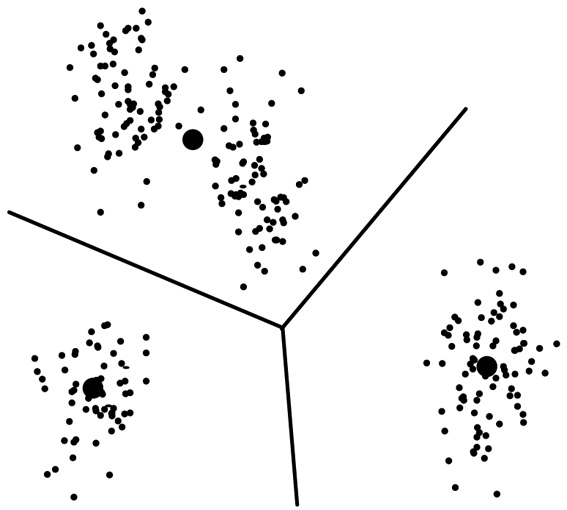
\includegraphics[width=5cm]{images/xmeans1.jpg}}\vspace{1mm}
  \subfloat[Selección punto de partida de K-Means ($k=2$).]{
   \label{f:step2}
    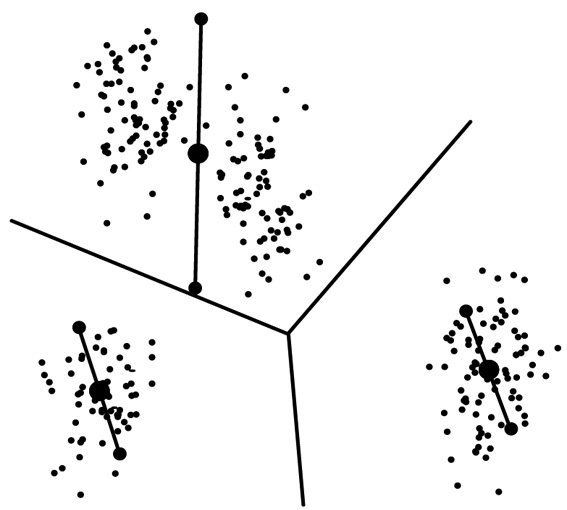
\includegraphics[width=5cm]{images/xmeans2.jpg}}\hspace{1mm}
  \subfloat[Resultado K-Means, evaluación BIC.]{
   \label{f:step3}
    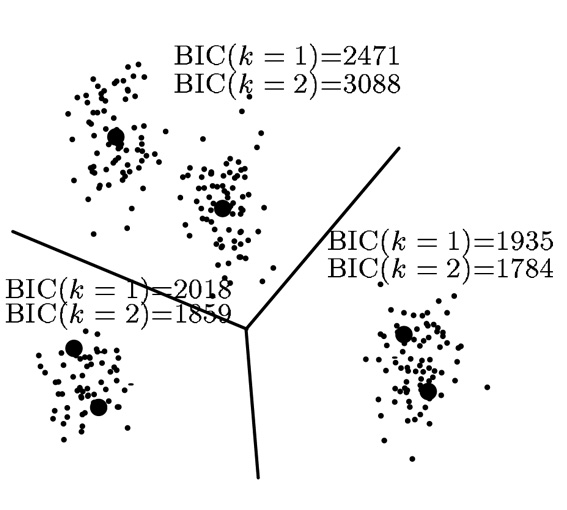
\includegraphics[width=5cm]{images/xmeans3.jpg}}\vspace{1mm}
  \subfloat[Resultado iteración X-Means]{
   \label{f:step4}
    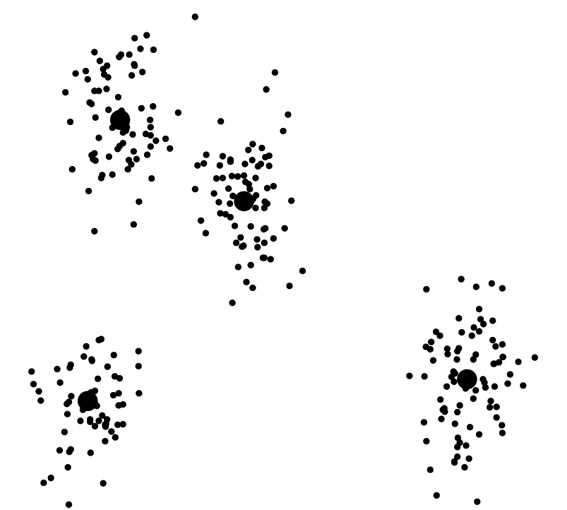
\includegraphics[width=5cm]{images/xmeans4.jpg}}
 \caption{Iteración X-Means.}
 \label{f:xmeans_steps}
\end{figure}

\subsection{Ventajas}

Una de las principales ventajas que posee este algoritmo radica en que es más escalable debido a que con cada iteración se reduce más el número de datos en los cuales K-Means se debe ejecutar, lo que hace que sea más fácil utilizarlo en conjuntos de datos de mayor tamaño. Otra ventaja es que se sabe que con K-Means de pocos clústers es menos probable incurrir en mínimos locales en comparación a uno realizado con muchos clústers. Por lo tanto, el hecho de que X-Means utilice un K-Means con $K=2$ favorece a que no se atasque en mínimos locales.

Además este método permite realizar una visualización del tipo árbol, la que crea una estructura jerárquica de los clústers.
%archivo implementacion
\chapter{Implementaci\'on}



%fin desarrollo

%archivo conclusiones
\chapter*{Conclusiones}
\addcontentsline{toc}{chapter}{Conclusiones}




%\backmatter
%\cleardoublepage

\singlespacing
\cleardoublepage

\bibliographystyle{plain}
\bibliography{bib/papers}

\end{document}